% Created by tikzDevice version 0.12.6 on 2026-03-25 11:39:47
% !TEX encoding = UTF-8 Unicode
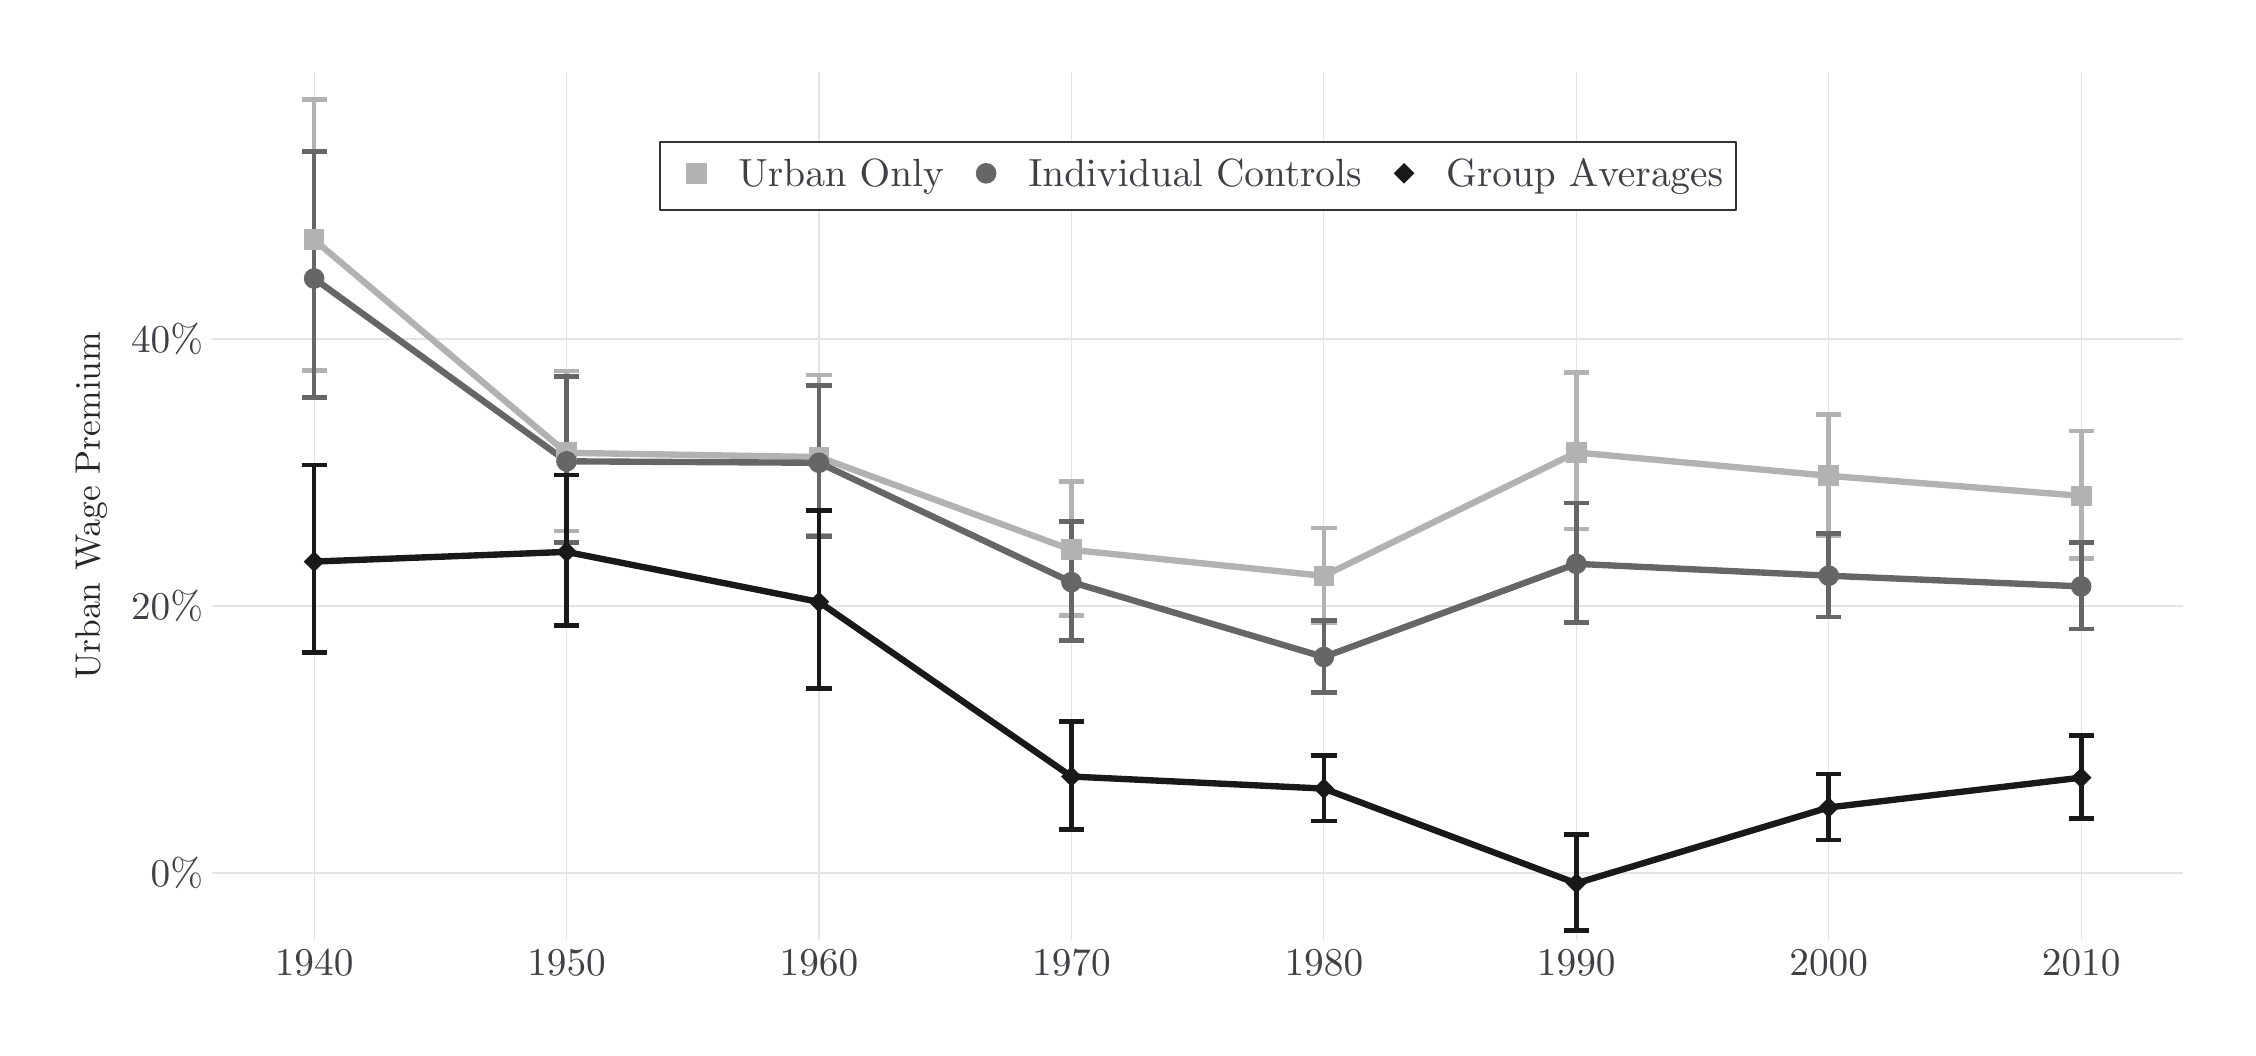
\begin{tikzpicture}[x=1pt,y=1pt]
\definecolor{fillColor}{RGB}{255,255,255}
\path[use as bounding box,fill=fillColor] (0,0) rectangle (794.97,361.35);
\begin{scope}
\path[clip] (  0.00,  0.00) rectangle (794.97,361.35);
\definecolor{drawColor}{RGB}{255,255,255}

\path[draw=drawColor,line width= 0.8pt,line join=round,line cap=round,fill=fillColor] (  0.00,  0.00) rectangle (794.97,361.35);
\end{scope}
\begin{scope}
\path[clip] ( 66.57, 31.76) rectangle (778.97,345.35);
\definecolor{drawColor}{RGB}{255,255,255}
\definecolor{fillColor}{RGB}{255,255,255}

\path[draw=drawColor,line width= 0.8pt,line join=round,line cap=round,fill=fillColor] ( 66.57, 31.76) rectangle (778.97,345.35);
\definecolor{drawColor}{RGB}{228,228,231}

\path[draw=drawColor,line width= 0.4pt,line join=round] ( 66.57, 55.88) --
	(778.97, 55.88);

\path[draw=drawColor,line width= 0.4pt,line join=round] ( 66.57,152.37) --
	(778.97,152.37);

\path[draw=drawColor,line width= 0.4pt,line join=round] ( 66.57,248.86) --
	(778.97,248.86);

\path[draw=drawColor,line width= 0.4pt,line join=round] (103.51, 31.76) --
	(103.51,345.35);

\path[draw=drawColor,line width= 0.4pt,line join=round] (194.73, 31.76) --
	(194.73,345.35);

\path[draw=drawColor,line width= 0.4pt,line join=round] (285.94, 31.76) --
	(285.94,345.35);

\path[draw=drawColor,line width= 0.4pt,line join=round] (377.16, 31.76) --
	(377.16,345.35);

\path[draw=drawColor,line width= 0.4pt,line join=round] (468.38, 31.76) --
	(468.38,345.35);

\path[draw=drawColor,line width= 0.4pt,line join=round] (559.59, 31.76) --
	(559.59,345.35);

\path[draw=drawColor,line width= 0.4pt,line join=round] (650.81, 31.76) --
	(650.81,345.35);

\path[draw=drawColor,line width= 0.4pt,line join=round] (742.03, 31.76) --
	(742.03,345.35);
\definecolor{drawColor}{gray}{0.70}

\path[draw=drawColor,line width= 2.3pt,line join=round] (103.51,284.69) --
	(194.73,207.72) --
	(285.94,206.19) --
	(377.16,172.68) --
	(468.38,163.25) --
	(559.59,207.86) --
	(650.81,199.42) --
	(742.03,192.17);
\definecolor{drawColor}{gray}{0.40}

\path[draw=drawColor,line width= 2.3pt,line join=round] (103.51,270.71) --
	(194.73,204.65) --
	(285.94,204.12) --
	(377.16,161.00) --
	(468.38,133.94) --
	(559.59,167.61) --
	(650.81,163.32) --
	(742.03,159.46);
\definecolor{drawColor}{gray}{0.10}

\path[draw=drawColor,line width= 2.3pt,line join=round] (103.51,168.42) --
	(194.73,171.92) --
	(285.94,153.84) --
	(377.16, 90.75) --
	(468.38, 86.39) --
	(559.59, 52.16) --
	(650.81, 79.58) --
	(742.03, 90.35);
\definecolor{drawColor}{gray}{0.70}

\path[draw=drawColor,line width= 1.7pt,line join=round] ( 98.95,335.31) --
	(108.07,335.31);

\path[draw=drawColor,line width= 1.7pt,line join=round] (103.51,335.31) --
	(103.51,237.43);

\path[draw=drawColor,line width= 1.7pt,line join=round] ( 98.95,237.43) --
	(108.07,237.43);
\definecolor{drawColor}{gray}{0.40}

\path[draw=drawColor,line width= 1.7pt,line join=round] ( 98.95,316.58) --
	(108.07,316.58);

\path[draw=drawColor,line width= 1.7pt,line join=round] (103.51,316.58) --
	(103.51,227.68);

\path[draw=drawColor,line width= 1.7pt,line join=round] ( 98.95,227.68) --
	(108.07,227.68);
\definecolor{drawColor}{gray}{0.10}

\path[draw=drawColor,line width= 1.7pt,line join=round] ( 98.95,203.33) --
	(108.07,203.33);

\path[draw=drawColor,line width= 1.7pt,line join=round] (103.51,203.33) --
	(103.51,135.44);

\path[draw=drawColor,line width= 1.7pt,line join=round] ( 98.95,135.44) --
	(108.07,135.44);
\definecolor{drawColor}{gray}{0.70}

\path[draw=drawColor,line width= 1.7pt,line join=round] (190.17,237.30) --
	(199.29,237.30);

\path[draw=drawColor,line width= 1.7pt,line join=round] (194.73,237.30) --
	(194.73,179.45);

\path[draw=drawColor,line width= 1.7pt,line join=round] (190.17,179.45) --
	(199.29,179.45);
\definecolor{drawColor}{gray}{0.40}

\path[draw=drawColor,line width= 1.7pt,line join=round] (190.17,235.39) --
	(199.29,235.39);

\path[draw=drawColor,line width= 1.7pt,line join=round] (194.73,235.39) --
	(194.73,175.34);

\path[draw=drawColor,line width= 1.7pt,line join=round] (190.17,175.34) --
	(199.29,175.34);
\definecolor{drawColor}{gray}{0.10}

\path[draw=drawColor,line width= 1.7pt,line join=round] (190.17,199.66) --
	(199.29,199.66);

\path[draw=drawColor,line width= 1.7pt,line join=round] (194.73,199.66) --
	(194.73,145.41);

\path[draw=drawColor,line width= 1.7pt,line join=round] (190.17,145.41) --
	(199.29,145.41);
\definecolor{drawColor}{gray}{0.70}

\path[draw=drawColor,line width= 1.7pt,line join=round] (281.38,235.87) --
	(290.50,235.87);

\path[draw=drawColor,line width= 1.7pt,line join=round] (285.94,235.87) --
	(285.94,177.84);

\path[draw=drawColor,line width= 1.7pt,line join=round] (281.38,177.84) --
	(290.50,177.84);
\definecolor{drawColor}{gray}{0.40}

\path[draw=drawColor,line width= 1.7pt,line join=round] (281.38,232.02) --
	(290.50,232.02);

\path[draw=drawColor,line width= 1.7pt,line join=round] (285.94,232.02) --
	(285.94,177.41);

\path[draw=drawColor,line width= 1.7pt,line join=round] (281.38,177.41) --
	(290.50,177.41);
\definecolor{drawColor}{gray}{0.10}

\path[draw=drawColor,line width= 1.7pt,line join=round] (281.38,186.93) --
	(290.50,186.93);

\path[draw=drawColor,line width= 1.7pt,line join=round] (285.94,186.93) --
	(285.94,122.54);

\path[draw=drawColor,line width= 1.7pt,line join=round] (281.38,122.54) --
	(290.50,122.54);
\definecolor{drawColor}{gray}{0.70}

\path[draw=drawColor,line width= 1.7pt,line join=round] (372.60,197.35) --
	(381.72,197.35);

\path[draw=drawColor,line width= 1.7pt,line join=round] (377.16,197.35) --
	(377.16,148.99);

\path[draw=drawColor,line width= 1.7pt,line join=round] (372.60,148.99) --
	(381.72,148.99);
\definecolor{drawColor}{gray}{0.40}

\path[draw=drawColor,line width= 1.7pt,line join=round] (372.60,183.00) --
	(381.72,183.00);

\path[draw=drawColor,line width= 1.7pt,line join=round] (377.16,183.00) --
	(377.16,139.79);

\path[draw=drawColor,line width= 1.7pt,line join=round] (372.60,139.79) --
	(381.72,139.79);
\definecolor{drawColor}{gray}{0.10}

\path[draw=drawColor,line width= 1.7pt,line join=round] (372.60,110.76) --
	(381.72,110.76);

\path[draw=drawColor,line width= 1.7pt,line join=round] (377.16,110.76) --
	(377.16, 71.49);

\path[draw=drawColor,line width= 1.7pt,line join=round] (372.60, 71.49) --
	(381.72, 71.49);
\definecolor{drawColor}{gray}{0.70}

\path[draw=drawColor,line width= 1.7pt,line join=round] (463.82,180.54) --
	(472.94,180.54);

\path[draw=drawColor,line width= 1.7pt,line join=round] (468.38,180.54) --
	(468.38,146.45);

\path[draw=drawColor,line width= 1.7pt,line join=round] (463.82,146.45) --
	(472.94,146.45);
\definecolor{drawColor}{gray}{0.40}

\path[draw=drawColor,line width= 1.7pt,line join=round] (463.82,147.04) --
	(472.94,147.04);

\path[draw=drawColor,line width= 1.7pt,line join=round] (468.38,147.04) --
	(468.38,121.13);

\path[draw=drawColor,line width= 1.7pt,line join=round] (463.82,121.13) --
	(472.94,121.13);
\definecolor{drawColor}{gray}{0.10}

\path[draw=drawColor,line width= 1.7pt,line join=round] (463.82, 98.41) --
	(472.94, 98.41);

\path[draw=drawColor,line width= 1.7pt,line join=round] (468.38, 98.41) --
	(468.38, 74.65);

\path[draw=drawColor,line width= 1.7pt,line join=round] (463.82, 74.65) --
	(472.94, 74.65);
\definecolor{drawColor}{gray}{0.70}

\path[draw=drawColor,line width= 1.7pt,line join=round] (555.03,236.81) --
	(564.15,236.81);

\path[draw=drawColor,line width= 1.7pt,line join=round] (559.59,236.81) --
	(559.59,180.18);

\path[draw=drawColor,line width= 1.7pt,line join=round] (555.03,180.18) --
	(564.15,180.18);
\definecolor{drawColor}{gray}{0.40}

\path[draw=drawColor,line width= 1.7pt,line join=round] (555.03,189.62) --
	(564.15,189.62);

\path[draw=drawColor,line width= 1.7pt,line join=round] (559.59,189.62) --
	(559.59,146.39);

\path[draw=drawColor,line width= 1.7pt,line join=round] (555.03,146.39) --
	(564.15,146.39);
\definecolor{drawColor}{gray}{0.10}

\path[draw=drawColor,line width= 1.7pt,line join=round] (555.03, 69.78) --
	(564.15, 69.78);

\path[draw=drawColor,line width= 1.7pt,line join=round] (559.59, 69.78) --
	(559.59, 35.17);

\path[draw=drawColor,line width= 1.7pt,line join=round] (555.03, 35.17) --
	(564.15, 35.17);
\definecolor{drawColor}{gray}{0.70}

\path[draw=drawColor,line width= 1.7pt,line join=round] (646.25,221.66) --
	(655.37,221.66);

\path[draw=drawColor,line width= 1.7pt,line join=round] (650.81,221.66) --
	(650.81,177.95);

\path[draw=drawColor,line width= 1.7pt,line join=round] (646.25,177.95) --
	(655.37,177.95);
\definecolor{drawColor}{gray}{0.40}

\path[draw=drawColor,line width= 1.7pt,line join=round] (646.25,178.66) --
	(655.37,178.66);

\path[draw=drawColor,line width= 1.7pt,line join=round] (650.81,178.66) --
	(650.81,148.38);

\path[draw=drawColor,line width= 1.7pt,line join=round] (646.25,148.38) --
	(655.37,148.38);
\definecolor{drawColor}{gray}{0.10}

\path[draw=drawColor,line width= 1.7pt,line join=round] (646.25, 91.65) --
	(655.37, 91.65);

\path[draw=drawColor,line width= 1.7pt,line join=round] (650.81, 91.65) --
	(650.81, 67.79);

\path[draw=drawColor,line width= 1.7pt,line join=round] (646.25, 67.79) --
	(655.37, 67.79);
\definecolor{drawColor}{gray}{0.70}

\path[draw=drawColor,line width= 1.7pt,line join=round] (737.47,215.65) --
	(746.59,215.65);

\path[draw=drawColor,line width= 1.7pt,line join=round] (742.03,215.65) --
	(742.03,169.55);

\path[draw=drawColor,line width= 1.7pt,line join=round] (737.47,169.55) --
	(746.59,169.55);
\definecolor{drawColor}{gray}{0.40}

\path[draw=drawColor,line width= 1.7pt,line join=round] (737.47,175.31) --
	(746.59,175.31);

\path[draw=drawColor,line width= 1.7pt,line join=round] (742.03,175.31) --
	(742.03,144.02);

\path[draw=drawColor,line width= 1.7pt,line join=round] (737.47,144.02) --
	(746.59,144.02);
\definecolor{drawColor}{gray}{0.10}

\path[draw=drawColor,line width= 1.7pt,line join=round] (737.47,105.53) --
	(746.59,105.53);

\path[draw=drawColor,line width= 1.7pt,line join=round] (742.03,105.53) --
	(742.03, 75.61);

\path[draw=drawColor,line width= 1.7pt,line join=round] (737.47, 75.61) --
	(746.59, 75.61);
\definecolor{fillColor}{gray}{0.70}

\path[fill=fillColor] ( 99.78,280.96) --
	(107.24,280.96) --
	(107.24,288.42) --
	( 99.78,288.42) --
	cycle;
\definecolor{fillColor}{gray}{0.40}

\path[fill=fillColor] (103.51,270.71) circle (  3.73);
\definecolor{fillColor}{gray}{0.10}

\path[fill=fillColor] ( 99.78,168.42) --
	(103.51,172.15) --
	(107.24,168.42) --
	(103.51,164.69) --
	cycle;
\definecolor{fillColor}{gray}{0.70}

\path[fill=fillColor] (191.00,203.99) --
	(198.46,203.99) --
	(198.46,211.45) --
	(191.00,211.45) --
	cycle;
\definecolor{fillColor}{gray}{0.40}

\path[fill=fillColor] (194.73,204.65) circle (  3.73);
\definecolor{fillColor}{gray}{0.10}

\path[fill=fillColor] (191.00,171.92) --
	(194.73,175.65) --
	(198.46,171.92) --
	(194.73,168.19) --
	cycle;
\definecolor{fillColor}{gray}{0.70}

\path[fill=fillColor] (282.21,202.46) --
	(289.67,202.46) --
	(289.67,209.92) --
	(282.21,209.92) --
	cycle;
\definecolor{fillColor}{gray}{0.40}

\path[fill=fillColor] (285.94,204.12) circle (  3.73);
\definecolor{fillColor}{gray}{0.10}

\path[fill=fillColor] (282.21,153.84) --
	(285.94,157.57) --
	(289.67,153.84) --
	(285.94,150.11) --
	cycle;
\definecolor{fillColor}{gray}{0.70}

\path[fill=fillColor] (373.43,168.95) --
	(380.89,168.95) --
	(380.89,176.41) --
	(373.43,176.41) --
	cycle;
\definecolor{fillColor}{gray}{0.40}

\path[fill=fillColor] (377.16,161.00) circle (  3.73);
\definecolor{fillColor}{gray}{0.10}

\path[fill=fillColor] (373.43, 90.75) --
	(377.16, 94.48) --
	(380.89, 90.75) --
	(377.16, 87.02) --
	cycle;
\definecolor{fillColor}{gray}{0.70}

\path[fill=fillColor] (464.65,159.52) --
	(472.11,159.52) --
	(472.11,166.98) --
	(464.65,166.98) --
	cycle;
\definecolor{fillColor}{gray}{0.40}

\path[fill=fillColor] (468.38,133.94) circle (  3.73);
\definecolor{fillColor}{gray}{0.10}

\path[fill=fillColor] (464.65, 86.39) --
	(468.38, 90.12) --
	(472.11, 86.39) --
	(468.38, 82.66) --
	cycle;
\definecolor{fillColor}{gray}{0.70}

\path[fill=fillColor] (555.86,204.13) --
	(563.32,204.13) --
	(563.32,211.59) --
	(555.86,211.59) --
	cycle;
\definecolor{fillColor}{gray}{0.40}

\path[fill=fillColor] (559.59,167.61) circle (  3.73);
\definecolor{fillColor}{gray}{0.10}

\path[fill=fillColor] (555.86, 52.16) --
	(559.59, 55.89) --
	(563.32, 52.16) --
	(559.59, 48.43) --
	cycle;
\definecolor{fillColor}{gray}{0.70}

\path[fill=fillColor] (647.08,195.69) --
	(654.54,195.69) --
	(654.54,203.15) --
	(647.08,203.15) --
	cycle;
\definecolor{fillColor}{gray}{0.40}

\path[fill=fillColor] (650.81,163.32) circle (  3.73);
\definecolor{fillColor}{gray}{0.10}

\path[fill=fillColor] (647.08, 79.58) --
	(650.81, 83.31) --
	(654.54, 79.58) --
	(650.81, 75.85) --
	cycle;
\definecolor{fillColor}{gray}{0.70}

\path[fill=fillColor] (738.30,188.44) --
	(745.76,188.44) --
	(745.76,195.90) --
	(738.30,195.90) --
	cycle;
\definecolor{fillColor}{gray}{0.40}

\path[fill=fillColor] (742.03,159.46) circle (  3.73);
\definecolor{fillColor}{gray}{0.10}

\path[fill=fillColor] (738.30, 90.35) --
	(742.03, 94.08) --
	(745.76, 90.35) --
	(742.03, 86.62) --
	cycle;
\end{scope}
\begin{scope}
\path[clip] (  0.00,  0.00) rectangle (794.97,361.35);
\definecolor{drawColor}{RGB}{63,63,70}

\node[text=drawColor,anchor=base east,inner sep=0pt, outer sep=0pt, scale=  1.42] at ( 63.37, 50.98) {0\%};

\node[text=drawColor,anchor=base east,inner sep=0pt, outer sep=0pt, scale=  1.42] at ( 63.37,147.47) {20\%};

\node[text=drawColor,anchor=base east,inner sep=0pt, outer sep=0pt, scale=  1.42] at ( 63.37,243.96) {40\%};
\end{scope}
\begin{scope}
\path[clip] (  0.00,  0.00) rectangle (794.97,361.35);
\definecolor{drawColor}{RGB}{63,63,70}

\node[text=drawColor,anchor=base,inner sep=0pt, outer sep=0pt, scale=  1.42] at (103.51, 18.76) {1940};

\node[text=drawColor,anchor=base,inner sep=0pt, outer sep=0pt, scale=  1.42] at (194.73, 18.76) {1950};

\node[text=drawColor,anchor=base,inner sep=0pt, outer sep=0pt, scale=  1.42] at (285.94, 18.76) {1960};

\node[text=drawColor,anchor=base,inner sep=0pt, outer sep=0pt, scale=  1.42] at (377.16, 18.76) {1970};

\node[text=drawColor,anchor=base,inner sep=0pt, outer sep=0pt, scale=  1.42] at (468.38, 18.76) {1980};

\node[text=drawColor,anchor=base,inner sep=0pt, outer sep=0pt, scale=  1.42] at (559.59, 18.76) {1990};

\node[text=drawColor,anchor=base,inner sep=0pt, outer sep=0pt, scale=  1.42] at (650.81, 18.76) {2000};

\node[text=drawColor,anchor=base,inner sep=0pt, outer sep=0pt, scale=  1.42] at (742.03, 18.76) {2010};
\end{scope}
\begin{scope}
\path[clip] (  0.00,  0.00) rectangle (794.97,361.35);
\definecolor{drawColor}{RGB}{39,39,42}

\node[text=drawColor,rotate= 90.00,anchor=base,inner sep=0pt, outer sep=0pt, scale=  1.28] at ( 26.06,188.55) {Urban Wage Premium};
\end{scope}
\begin{scope}
\path[clip] (  0.00,  0.00) rectangle (794.97,361.35);
\definecolor{drawColor}{gray}{0.20}
\definecolor{fillColor}{RGB}{255,255,255}

\path[draw=drawColor,line width= 0.8pt,line join=round,line cap=round,fill=fillColor] (228.37,295.49) rectangle (617.17,319.95);
\end{scope}
\begin{scope}
\path[clip] (  0.00,  0.00) rectangle (794.97,361.35);
\definecolor{drawColor}{RGB}{255,255,255}
\definecolor{fillColor}{RGB}{255,255,255}

\path[draw=drawColor,line width= 0.8pt,line join=round,line cap=round,fill=fillColor] (234.37,301.49) rectangle (248.83,315.95);
\definecolor{fillColor}{gray}{0.70}

\path[fill=fillColor] (237.87,304.99) --
	(245.33,304.99) --
	(245.33,312.45) --
	(237.87,312.45) --
	cycle;
\end{scope}
\begin{scope}
\path[clip] (  0.00,  0.00) rectangle (794.97,361.35);
\definecolor{drawColor}{RGB}{255,255,255}
\definecolor{fillColor}{RGB}{255,255,255}

\path[draw=drawColor,line width= 0.8pt,line join=round,line cap=round,fill=fillColor] (339.11,301.49) rectangle (353.56,315.95);
\definecolor{fillColor}{gray}{0.40}

\path[fill=fillColor] (346.33,308.72) circle (  3.73);
\end{scope}
\begin{scope}
\path[clip] (  0.00,  0.00) rectangle (794.97,361.35);
\definecolor{drawColor}{RGB}{255,255,255}
\definecolor{fillColor}{RGB}{255,255,255}

\path[draw=drawColor,line width= 0.8pt,line join=round,line cap=round,fill=fillColor] (490.12,301.49) rectangle (504.58,315.95);
\definecolor{fillColor}{gray}{0.10}

\path[fill=fillColor] (493.62,308.72) --
	(497.35,312.45) --
	(501.08,308.72) --
	(497.35,304.99) --
	cycle;
\end{scope}
\begin{scope}
\path[clip] (  0.00,  0.00) rectangle (794.97,361.35);
\definecolor{drawColor}{RGB}{63,63,70}

\node[text=drawColor,anchor=base west,inner sep=0pt, outer sep=0pt, scale=  1.42] at (256.83,303.82) {Urban Only};
\end{scope}
\begin{scope}
\path[clip] (  0.00,  0.00) rectangle (794.97,361.35);
\definecolor{drawColor}{RGB}{63,63,70}

\node[text=drawColor,anchor=base west,inner sep=0pt, outer sep=0pt, scale=  1.42] at (361.56,303.82) {Individual Controls};
\end{scope}
\begin{scope}
\path[clip] (  0.00,  0.00) rectangle (794.97,361.35);
\definecolor{drawColor}{RGB}{63,63,70}

\node[text=drawColor,anchor=base west,inner sep=0pt, outer sep=0pt, scale=  1.42] at (512.58,303.82) {Group Averages};
\end{scope}
\end{tikzpicture}
